\PassOptionsToPackage{unicode}{hyperref}
\documentclass[aspectratio=1610, professionalfonts, 9pt]{beamer}

\usefonttheme[onlymath]{serif}
\usetheme[showtotalframes]{tudo}

\ifluatex
  \usepackage{polyglossia}
  \setmainlanguage{german}
\else
  \ifxetex
    \usepackage{polyglossia}
    \setmainlanguage{german}
  \else
    \usepackage[german]{babel}
  \fi
\fi


% Mathematik
\usepackage{amsmath}
\usepackage{amssymb}
\usepackage{mathtools}
\usepackage{cancel}

\usepackage{hyperref}
\usepackage{bookmark}
\usepackage{siunitx}
\usepackage{pdfpages}
\usepackage{booktabs}
\usepackage{subcaption}

%%%%%%%%%%%%%%%%%%%%%%%%%%%%%%%%%%%%%%%%%%%%%%%%%%%%%%%%%%%%%%%%%%%%%%%%%%%%%%%%
%%%%%-------------Hier Titel/Autor/Grafik/Lehrstuhl eintragen--------------%%%%%
%%%%%%%%%%%%%%%%%%%%%%%%%%%%%%%%%%%%%%%%%%%%%%%%%%%%%%%%%%%%%%%%%%%%%%%%%%%%%%%%

%Titel:
\title{Klassifikation von Erkrankungen der Retina anhand von OCT Bildern}
%Autor
% \author[Sedlaczek, Wendland]{Kevin Sedlaczek, Björn Wendland}
%Lehrstuhl/Fakultät
\institute[E4/5]{TU Dortmund \\  Physik}
%Titelgrafik
\titlegraphic{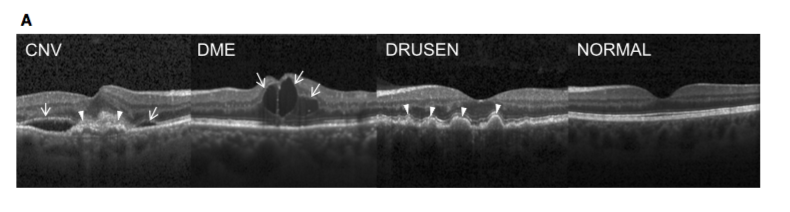
\includegraphics[width=0.95\textwidth]{images/title.png}}


\begin{document}

\maketitle

\begin{frame}{Aufgabenstellung}
  \begin{block}{Fragestellung}
    \centering
    Lässt sich der Zustand einer menschlichen Retina anhand von OCT-Bildern in die 4 Klassen
    %
    \begin{equation*}
        [\text{NORMAL}, \text{CNV}, \text{DRUSEN}, \text{DME}]
    \end{equation*}
    %
    einteilen und somit eine Diagnose mit Hilfe von ML stellen? \\
    \textit{choroidal neovascularization}, \textit{macular edema}, \textit{drusen}
  \begin{itemize}
    \item CNV: \textit{Bildung neuer Blutgefäße im Auge}
    \item DRUSEN: \textit{Ablagerung von proteinhaltigem Material, das verkalkt}
    \item DME: \textit{Ansammlung extrazellulärer Flüssigkeit im Bereich des menschlichen Auges}
  \end{itemize}
  \end{block}
  \begin{itemize}
    \item \textit{optical coherence tomography}: hoch auflösende Bildgebung von Retina Querschnitten lebender Patienten
    \item Analyse durch erfahrenen Mediziner notwendig
    \item Idee: Methoden maschinellen Lernens um Krankheiten zu erkennen
  \end{itemize}
\end{frame}

\begin{frame}
    \frametitle{Datensatz}
    \centering
    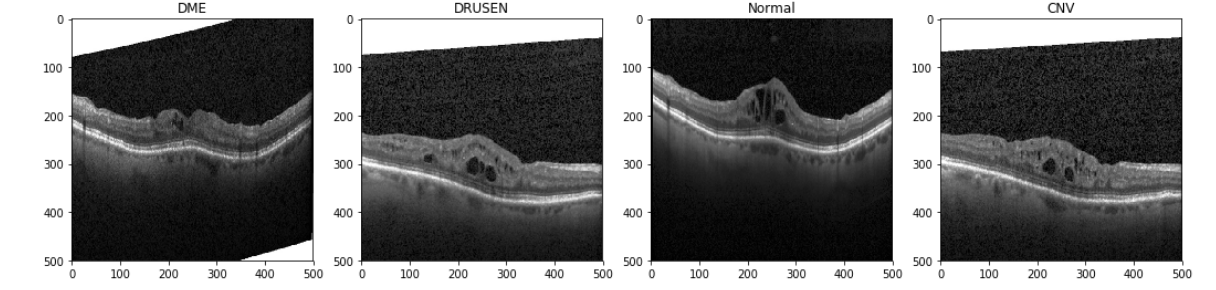
\includegraphics[width=0.9\textwidth]{images/examples.png}\\
    \begin{itemize}
        \item Inhalt: 84,495 Röntgen Bilder ($500\times500$px JPEG) aufgeteilt in 4 Klassen (Erkrankungen + gesund)
    \end{itemize}
\end{frame}

\begin{frame}
    \frametitle{Verteilung auf die Klassen}
    \centering
    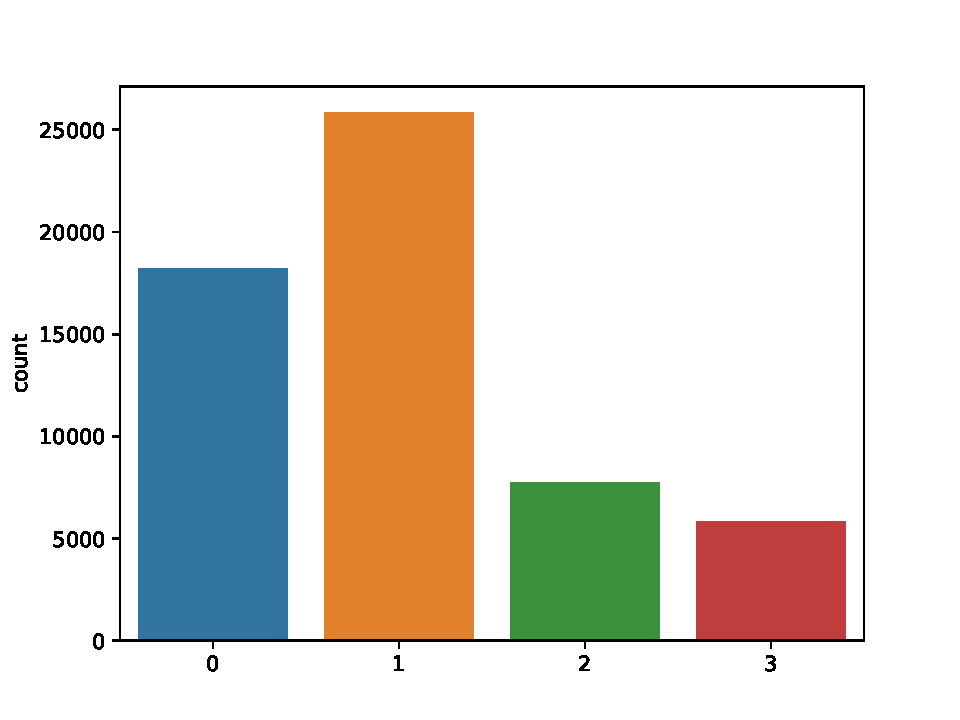
\includegraphics[width=0.6\textwidth]{images/countplot_relu.pdf}\\
\end{frame}

\begin{frame}
    \frametitle{Architektur des Netzes}
    \begin{itemize}
        \item 2 (Convolutional 2D layer + MaxPooling2D layer) \textit{Pakete} (64/32 Filter)
        \item Kernel sizes: (4, 4) / (3, 3)
    \end{itemize}
    Übergang zu Fully connected layern
    \begin{itemize}
        \item Dropout mit rate=$0.25$
        \item Dense layer: Aktivierungsfunktion \textbf{elu}
        \item Filter: $1000$, $250$, $100$, $32$, $4$
        \item Unterbrochen von einem flatten layer und weiterem Dropout (rate=$0.5$)
        \item Output layer: 4 Filter mit Aktivierungsfunktion \textit{softmax}
    \end{itemize}
\end{frame}

\begin{frame}
    \frametitle{Architektur des Netzes}
    \begin{table}[htb]
        \centering
        \begin{tabular}{l
                        l
                        l}
            \toprule
            Layer (type)                      & Output Shape     & Anzahl Parameter      \\
            \midrule
            Conv 2D         & (None, 199, 199, 64)  & 1088 \\
            Max Pooling 2D  & (None, 66, 66, 64)    & 0 \\
            Conv 2D         & (None, 32, 32, 32)    & 32800 \\
            Max Pooling 2D  & (None, 10, 10, 32)    & 0 \\
            Dropout         & (None, 10, 10, 32)    & 0 \\
            Dense           & (None, 10, 10, 1000)  & 33000 \\
            Dense           & (None, 10, 10, 250)   & 250250 \\
            Flatten         & (None, 25000)         & 0 \\
            Dense           & (None, 100)           & 2500100 \\
            Dropout         & (None, 100)           & 0 \\
            Dense           & (None, 32)            & 3232 \\
            Dense           & (None, 4)             & 132 \\
            \midrule
            Total           &                       & 2820602 \\
            \bottomrule
        \end{tabular}
    \end{table}
\end{frame}

{
    \setbeamercolor{background canvas}{bg=}
    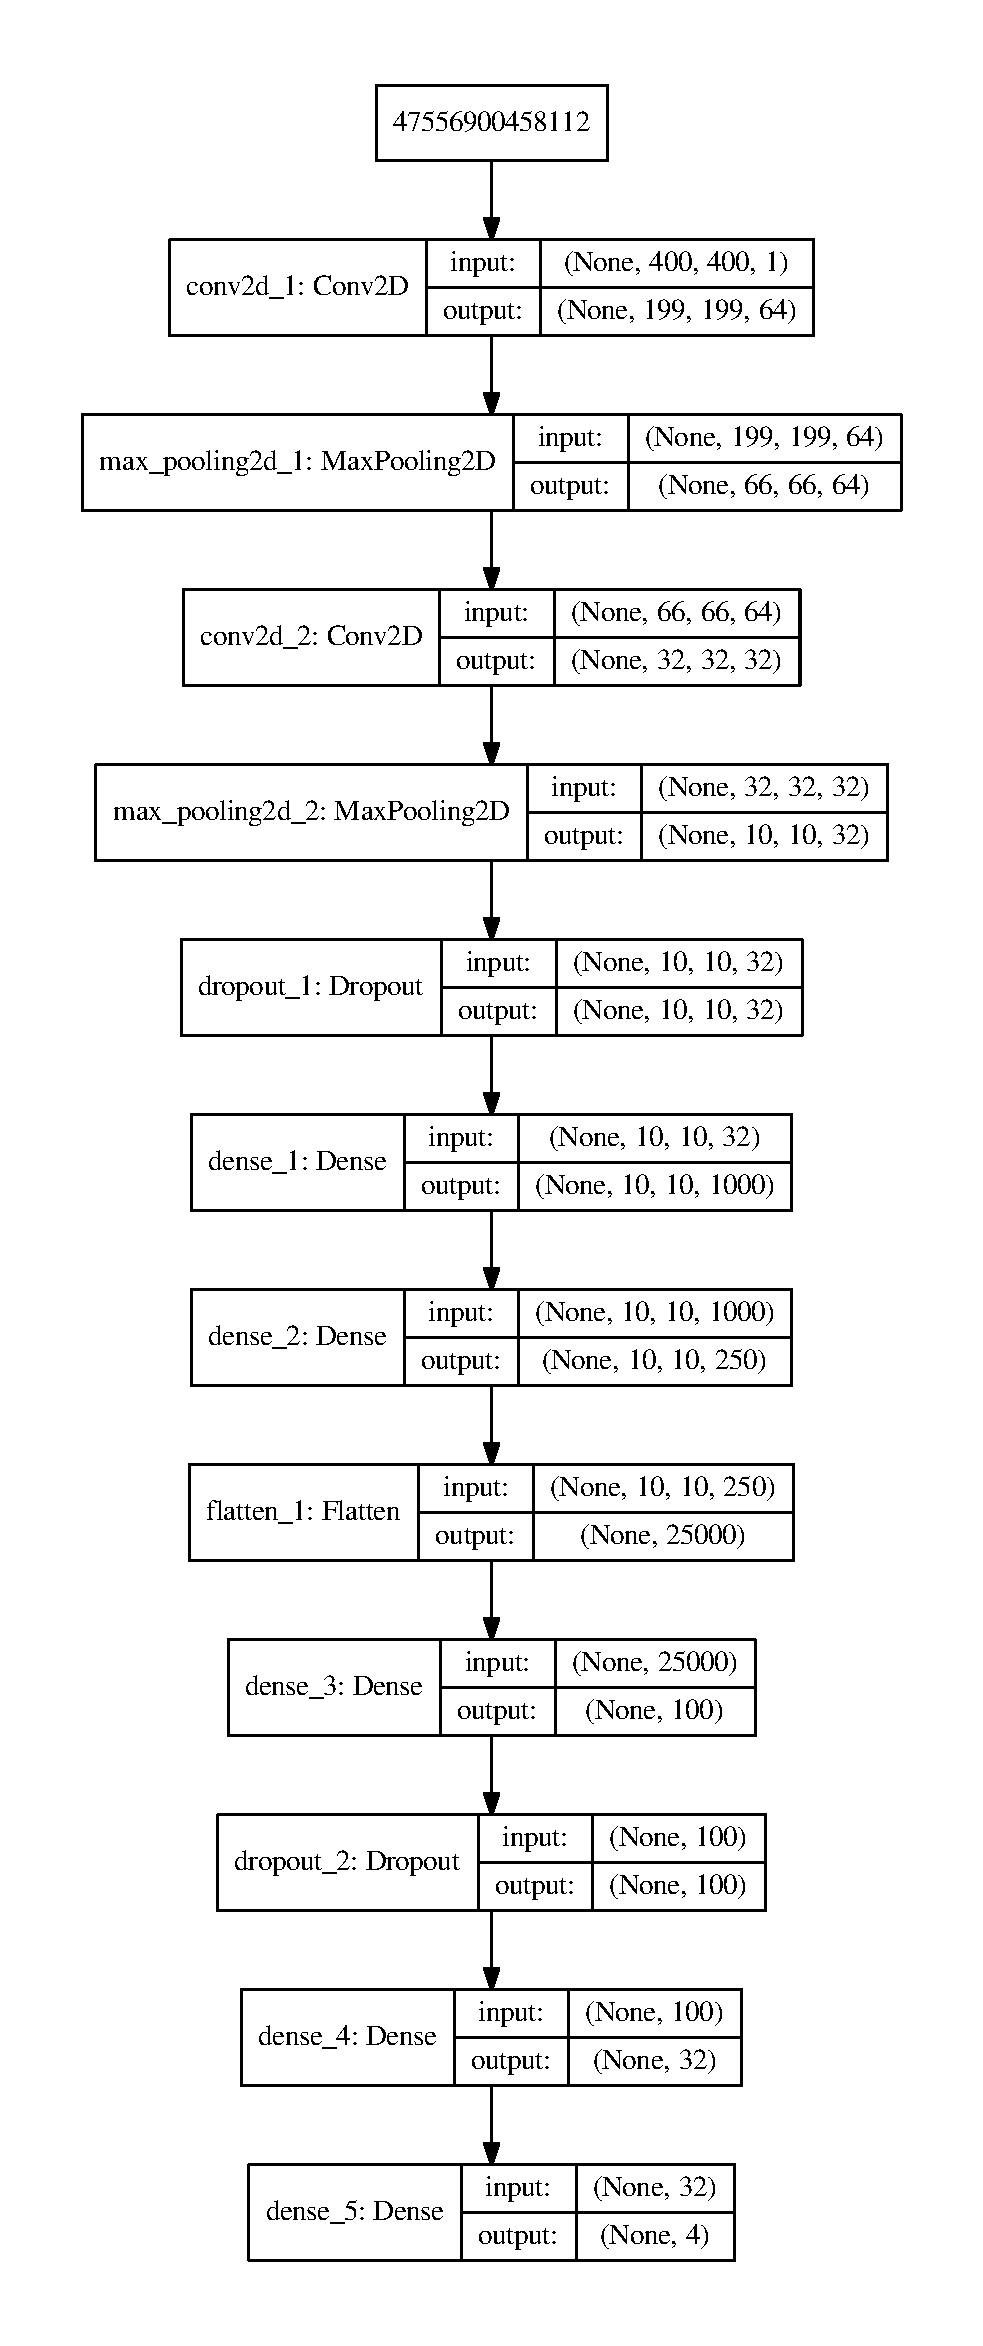
\includepdf[pages=1]{images/network.pdf}

}
\begin{frame}
    \frametitle{Ergebnisse Convolutional network}
    \begin{figure}[H]%
        \begin{subfigure}{0.3\textwidth}%
            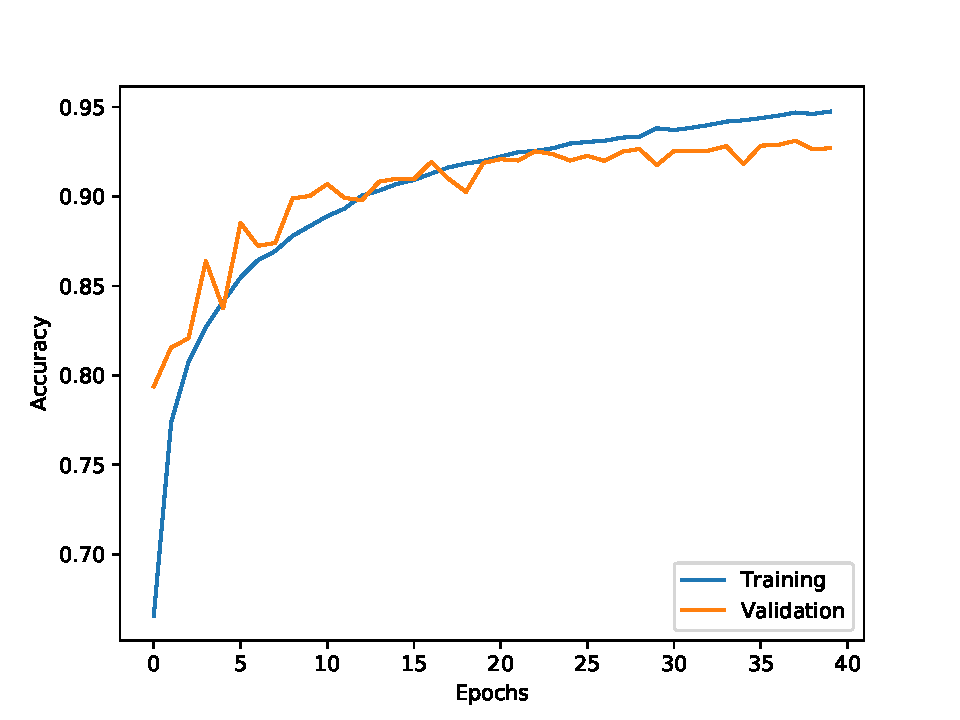
\includegraphics[width=1.2\linewidth]{images/accuracy_history_elu.pdf}%
            \caption{elu whole}%
        \end{subfigure}%
        \hfill%
        \begin{subfigure}{0.3\textwidth}%
            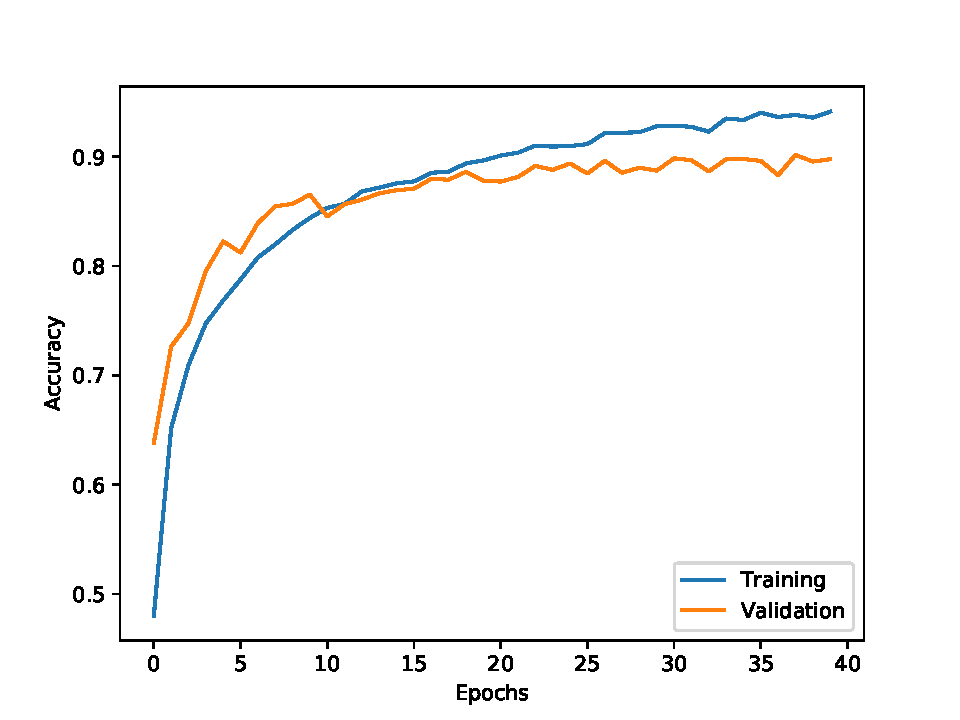
\includegraphics[width=1.2\linewidth]{images/accuracy_history_equal.pdf}%
            \caption{elu equal}%
        \end{subfigure}%
        \hfill%
        \begin{subfigure}{0.3\textwidth}%
            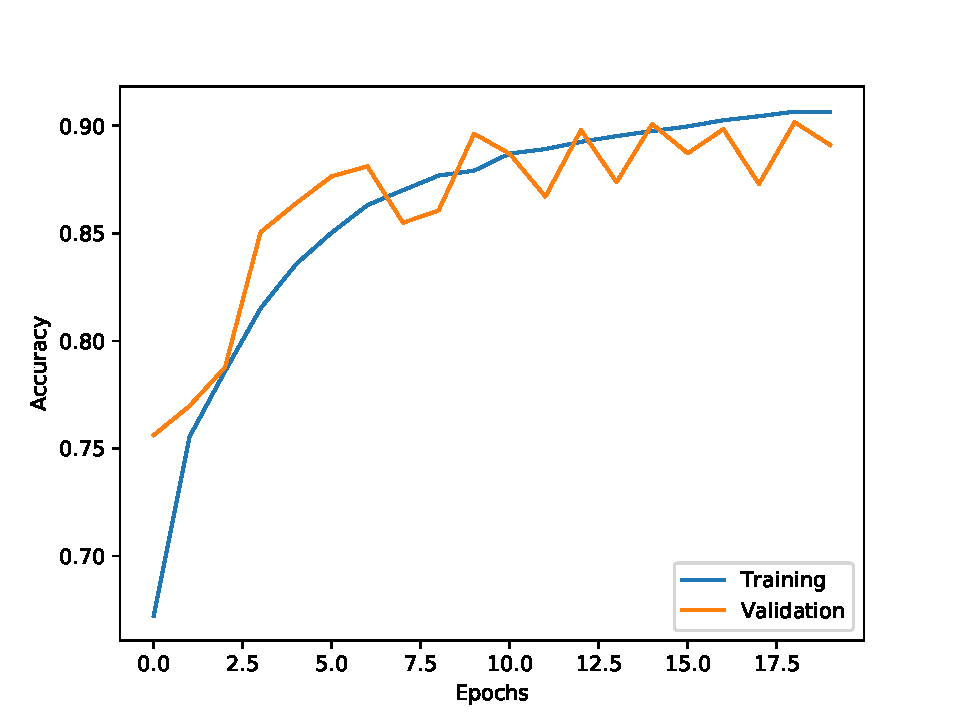
\includegraphics[width=1.2\linewidth]{images/accuracy_history_relu.pdf}%
            \caption{relu}%
        \end{subfigure}%
    \end{figure}%
\end{frame}

\begin{frame}
    \frametitle{Ergebnisse Convolutional network}
    \begin{figure}[H]%
        \begin{subfigure}{0.3\textwidth}%
            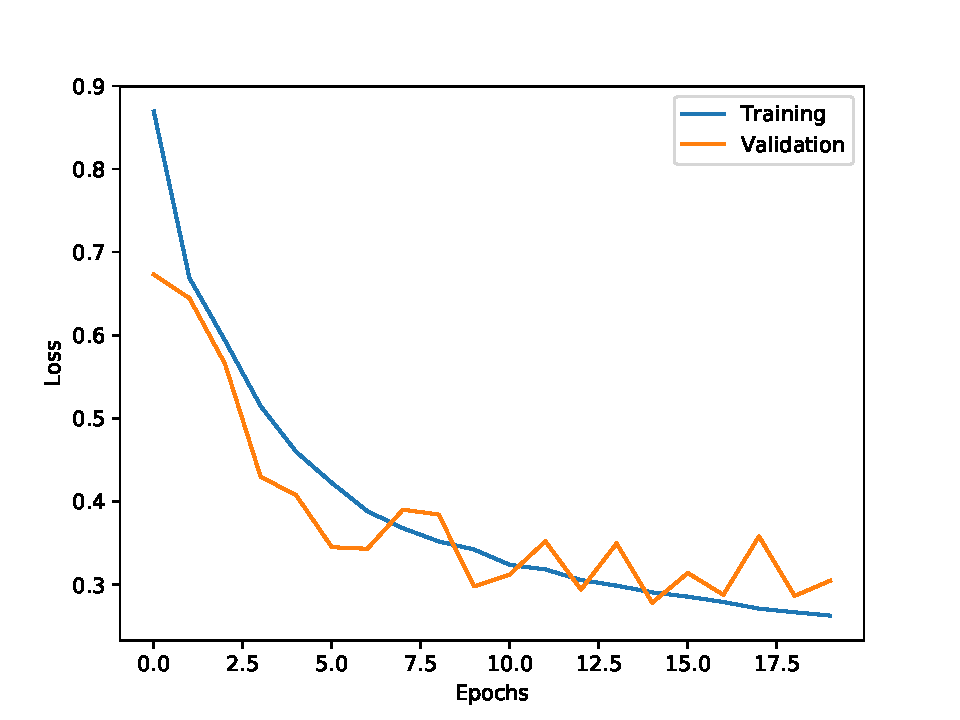
\includegraphics[width=1.2\linewidth]{images/loss_history_relu.pdf}%
            \caption{relu}%
        \end{subfigure}%
        \hfill%
        \begin{subfigure}{0.3\textwidth}%
            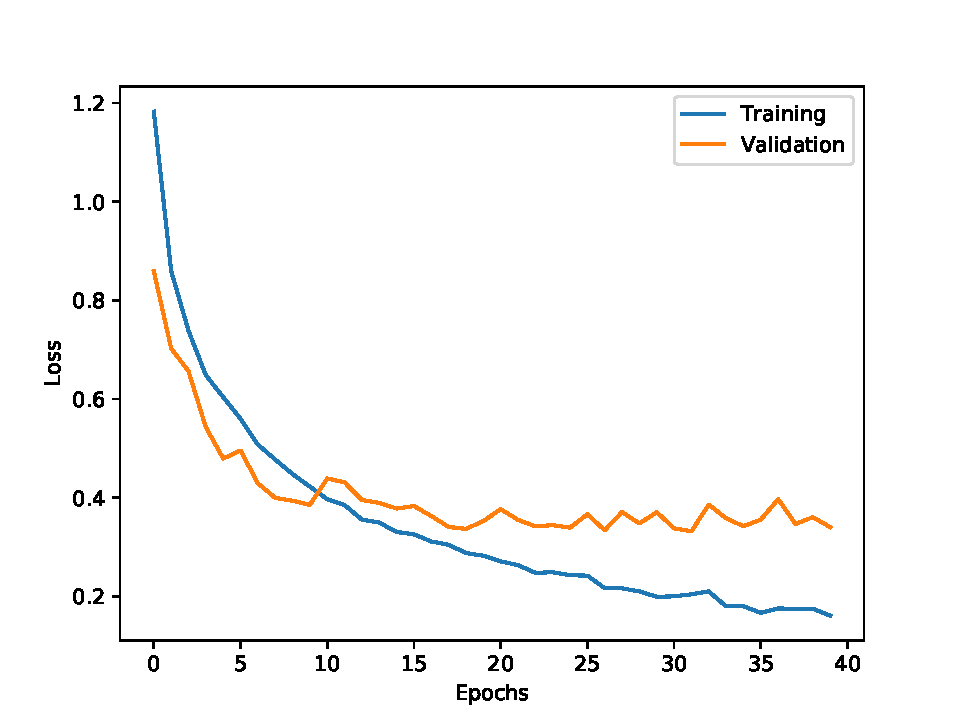
\includegraphics[width=1.2\linewidth]{images/loss_history_equal.pdf}%
            \caption{elu equal}%
        \end{subfigure}%
        \hfill%
        \begin{subfigure}{0.3\textwidth}%
            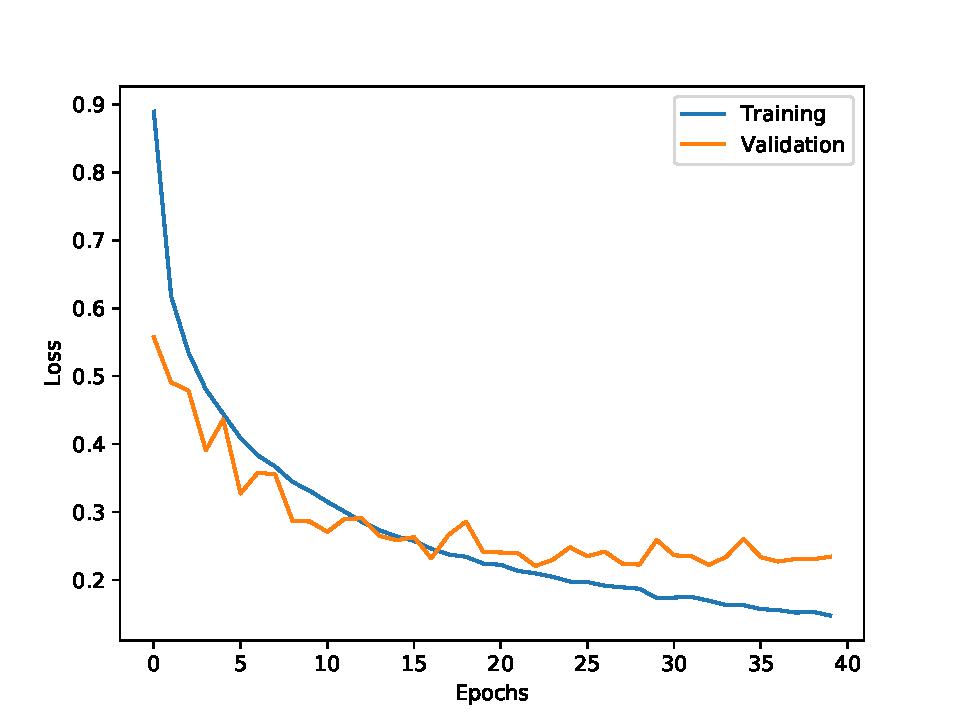
\includegraphics[width=1.2\linewidth]{images/loss_history_elu.pdf}%
            \caption{elu}%
        \end{subfigure}%
    \end{figure}%
\end{frame}

\begin{frame}
    \frametitle{Ergebnisse Convolutional network}
    \begin{figure}[H]%
        \begin{subfigure}{0.3\textwidth}%
            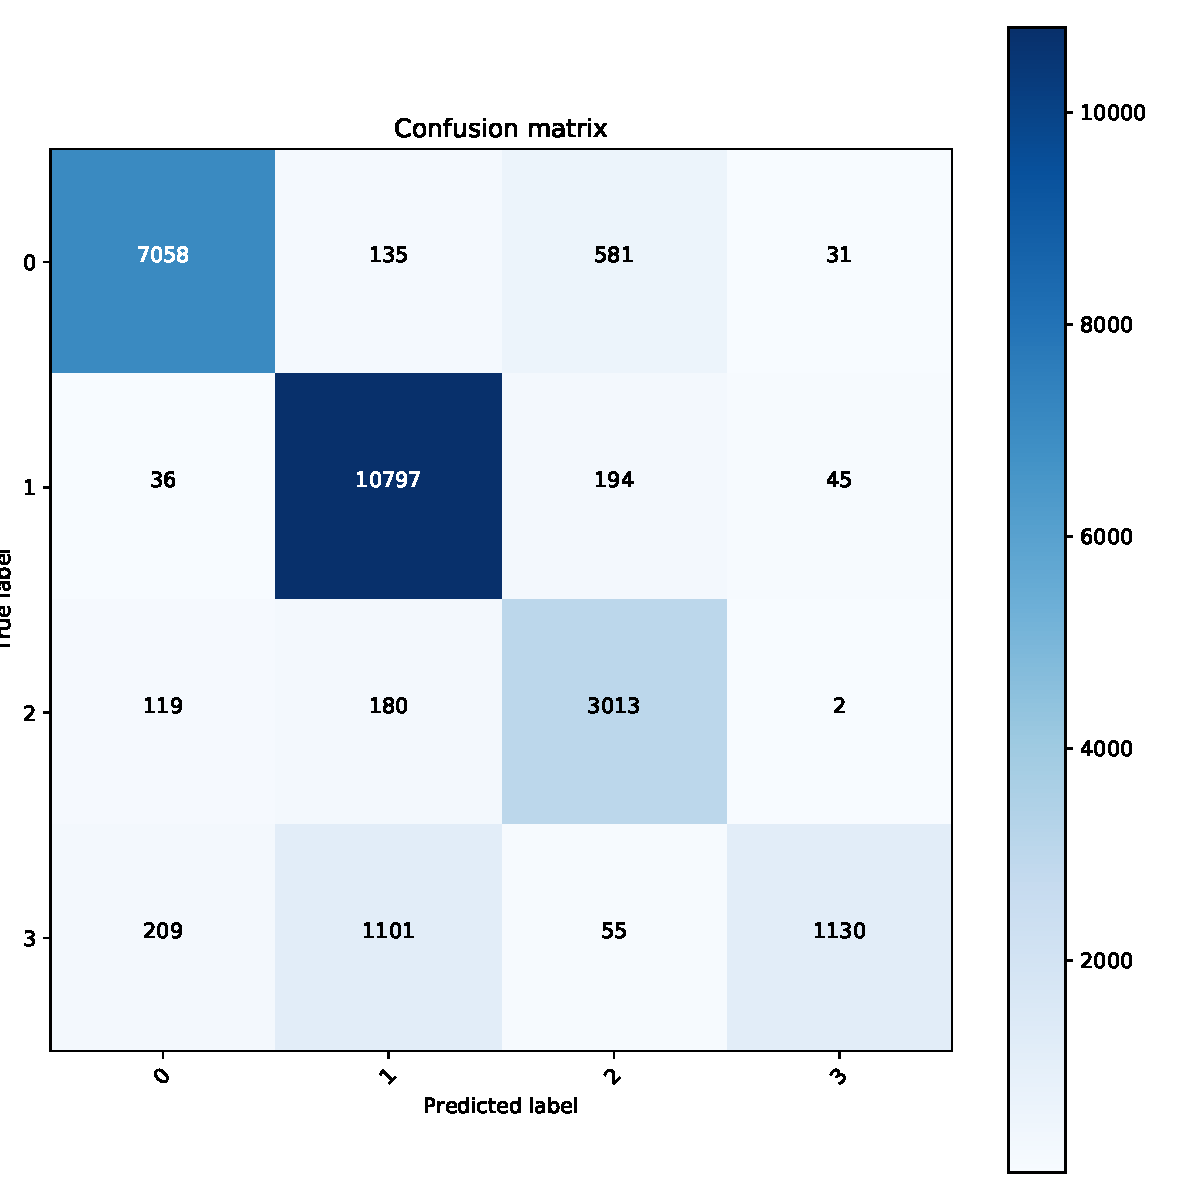
\includegraphics[width=1.2\linewidth]{images/confusion_matrix_relu.pdf}%
            \caption{relu}%
        \end{subfigure}%
        \hfill%
        \begin{subfigure}{0.3\textwidth}%
            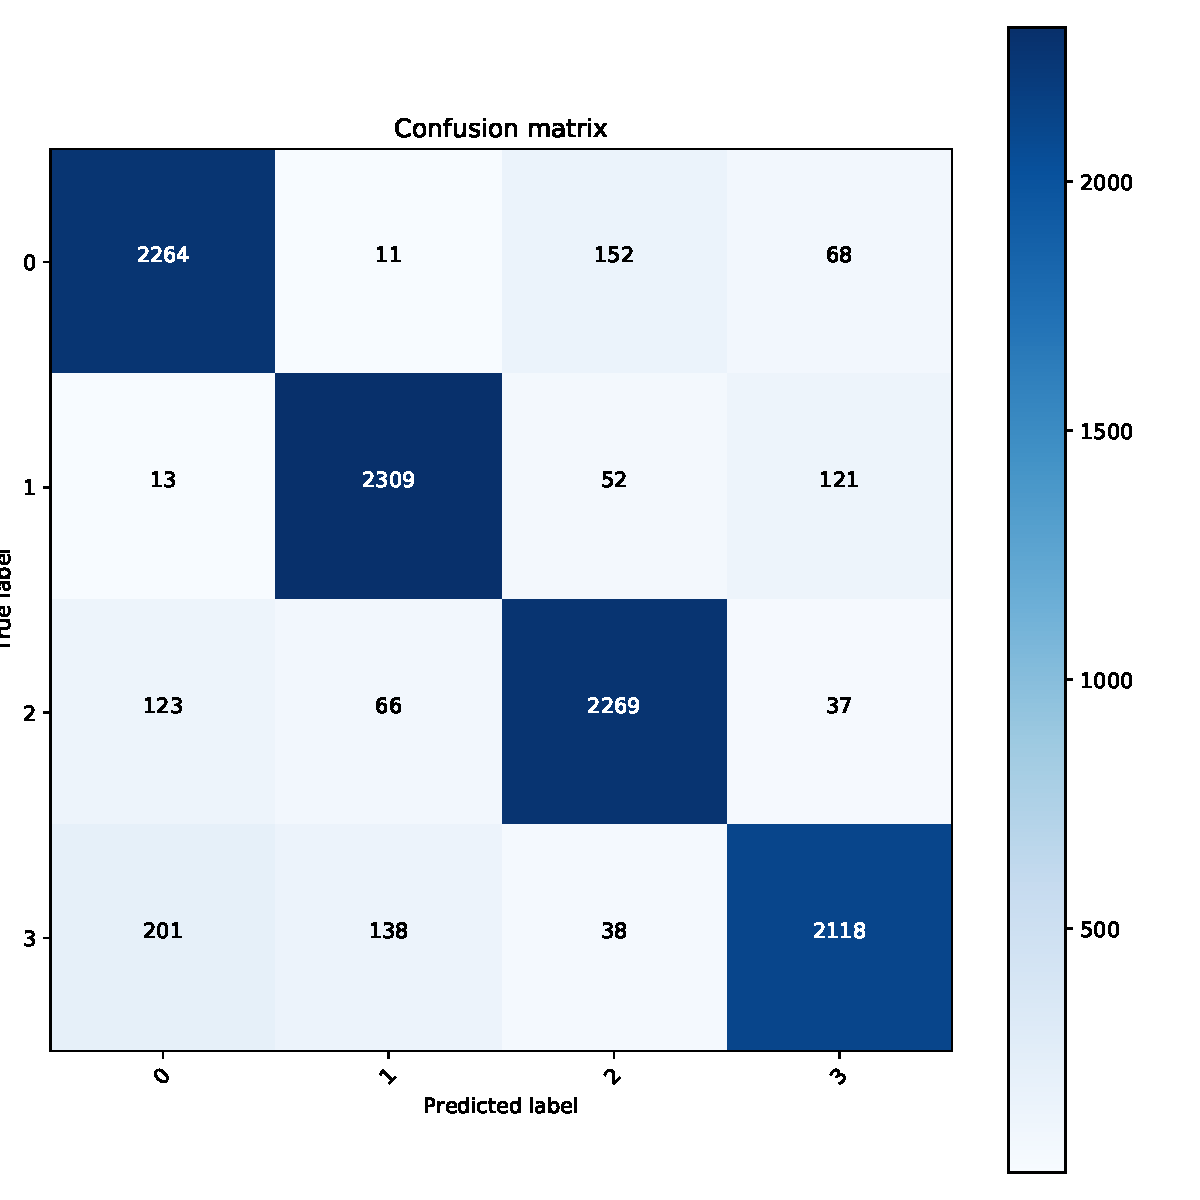
\includegraphics[width=1.2\linewidth]{images/confusion_matrix_equal.pdf}%
            \caption{elu equal}%
        \end{subfigure}%
        \hfill%
        \begin{subfigure}{0.3\textwidth}%
            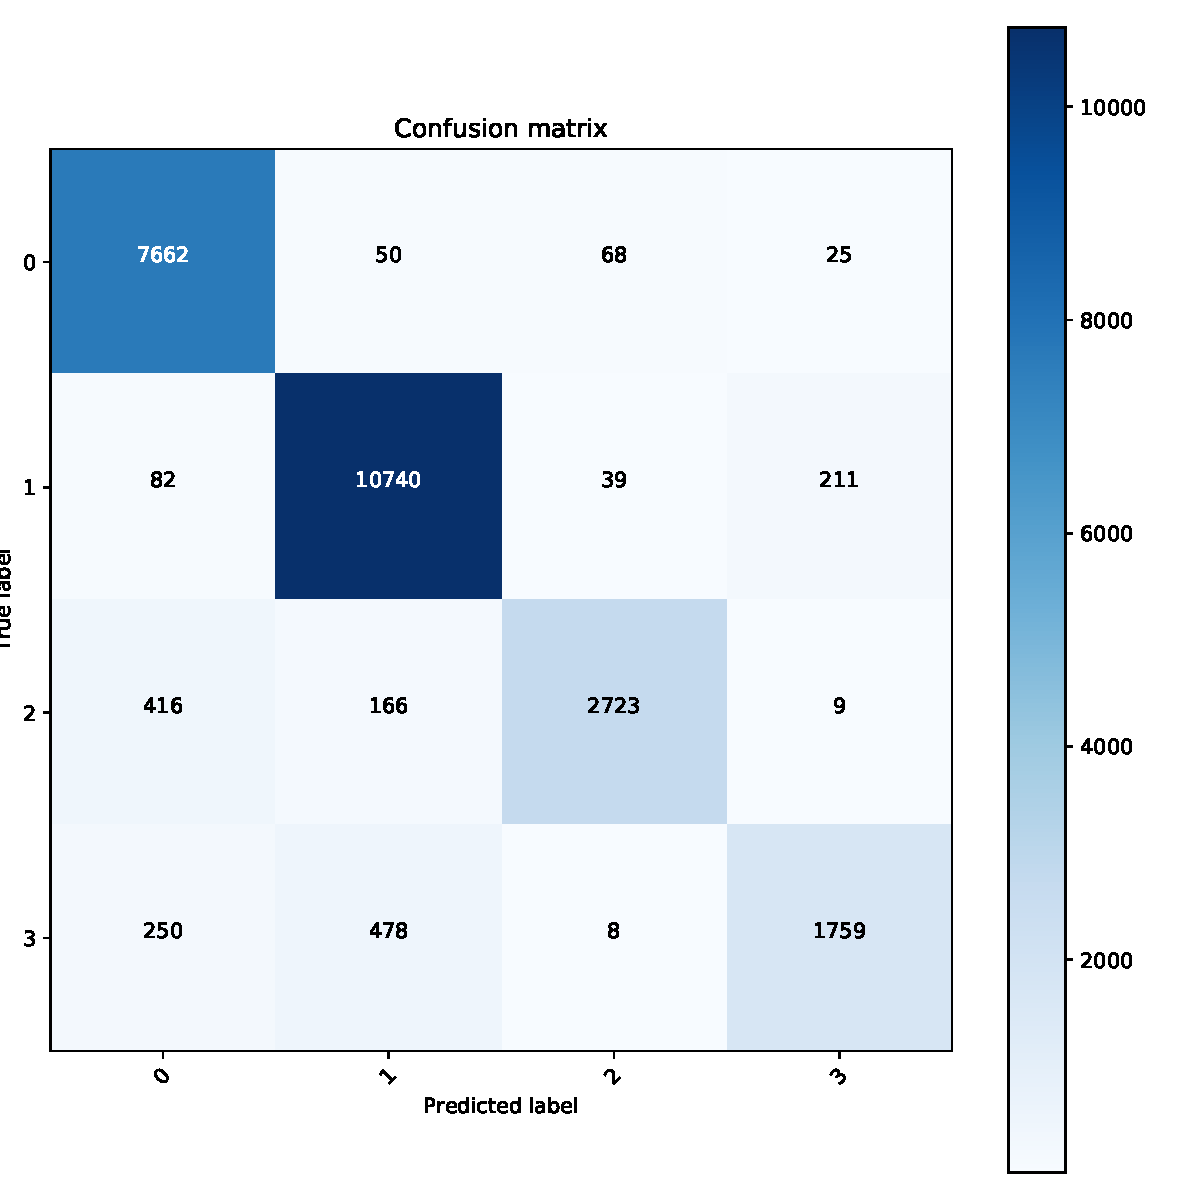
\includegraphics[width=1.2\linewidth]{images/confusion_matrix_elu.pdf}%
            \caption{elu}%
        \end{subfigure}%
    \end{figure}%
\end{frame}


\begin{frame}
\frametitle{Alternative Methode}

\begin{itemize}
 \item[\textbullet] Datenvorbereitung:
 \begin{itemize}
  \item Gelabelte Bilder (50,100) in hdf5-Format abgespeichert
  \item Feinere Krönung bringt keine Verbesserung!
  \item Gewichte für jedes Bild $\Rightarrow$ Ausgleich der Unterschiede der Klassenmenge
 \end{itemize}
\end{itemize}
\vspace{0.5cm}

\begin{itemize}
 \item[\textbullet] Drei Ansätze:
 \begin{itemize}
  \item Füttere Pixel nacheinander ins neuronale Netz ($\Rightarrow$ (zu) viele Inputfeature Bilder größer als (50,100))
  \item Berechne sowohl in $x$- und $y$-Richtung die Mittelwerte aller Pixel einer Linie ((100,100) Bild $\rightarrow$ 200 Werte)
  \item Definiere Fenster und berechne Mittelwerte der im Fenster liegenden Pixel ((50,100) abgerastert mit (2,4) Fenster $\Rightarrow$ 625 Inputfeature)
 \end{itemize}
\vspace{0.5cm}
\item[\textbullet] Letzte Methode am vielversprechendsten!
\vspace{0.5cm}
\item[\textbullet] Werte eines Bildes werden auf den maximalen Wert eines Bildes normiert
\end{itemize}
\end{frame}

\begin{frame}
 \frametitle{Referenzstruktur des Neuronalen Netzes}
 \begin{columns}
  \column{7cm}
   \begin{itemize}
  \item[\textbullet] Vollständig vernetztes NN bestehend aus Dense Layer
  \item[\textbullet] Festgelegte Referenzstruktur $\Rightarrow$
  \item[\textbullet] Dropoutrates:
  \begin{itemize}
   \item Nach 1. Layer: 0.5
   \item Nach 2. Layer: 0.4
   \item Nach 3. Layer: 0.3
   \item Nach 4. Layer: 0.2
   \item Nach 5. Layer: 0.2
  \end{itemize}
  \item[\textbullet] Aktivierungsfunktionen:
  \begin{itemize}
   \item Hidden Layer: relu
   \item Outputlayer: softmax
  \end{itemize}
  \item[\textbullet] Loss-Funktion: Kategorische Entropie
  \item[\textbullet] Adam mit angepasster Lernrate von 0.0001 als Optimierer
  \item[\textbullet] 150 Epochen mit einer Batchgröße von 100
 \end{itemize}
  \column{3cm}
  \vspace{-1cm}
  \begin{figure}
   \centering
   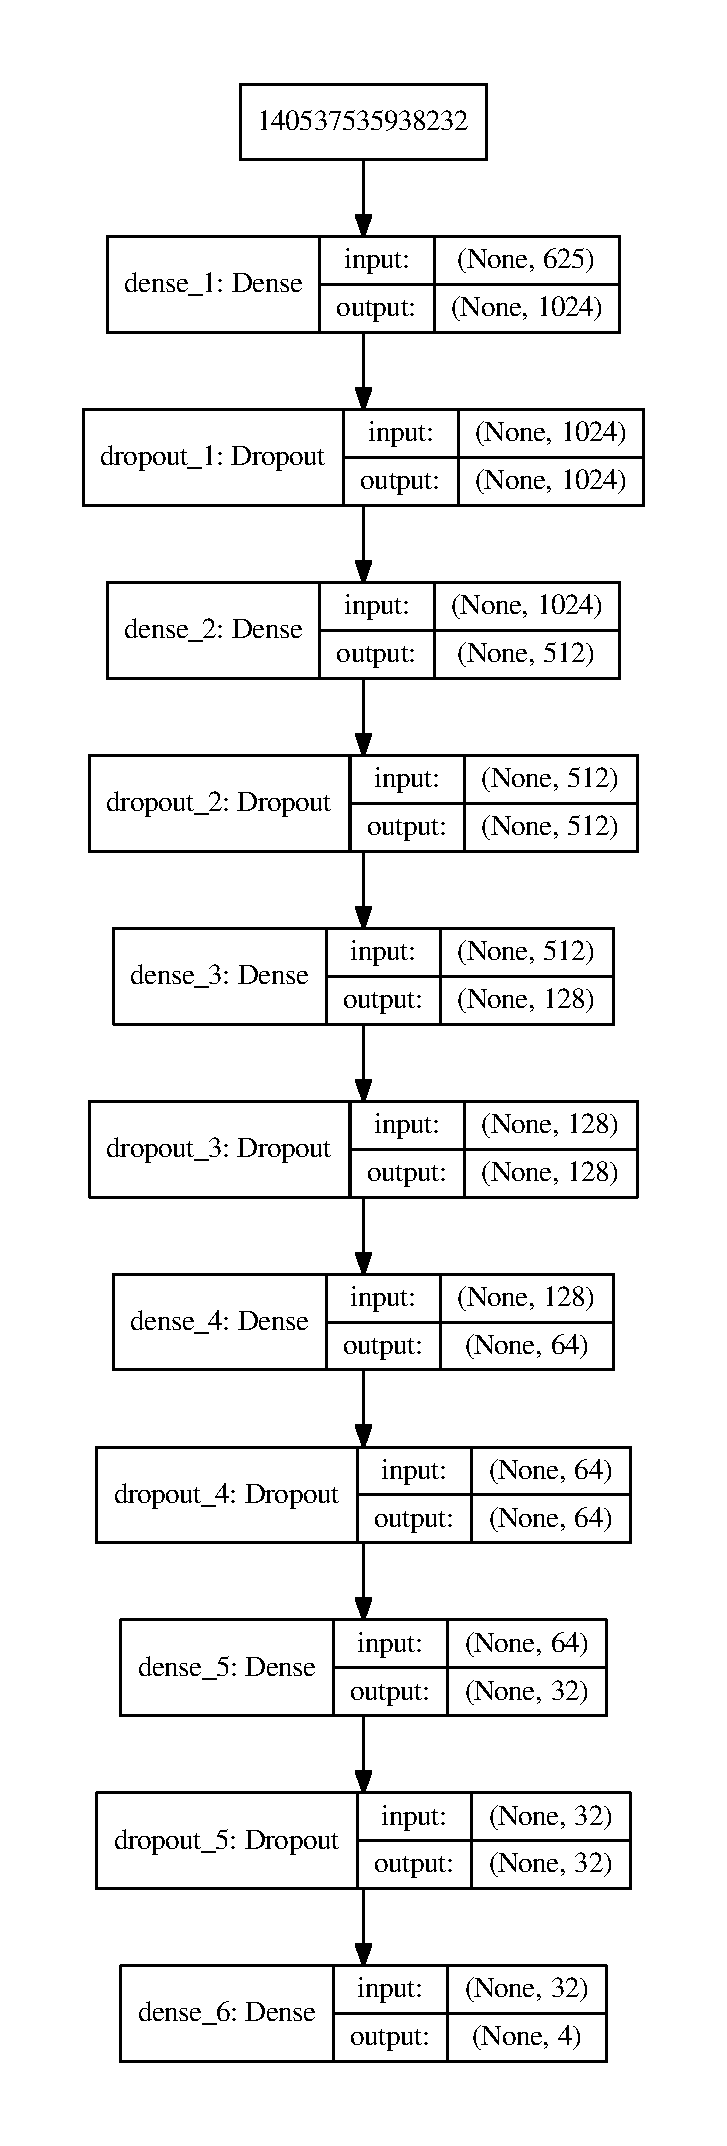
\includegraphics[width=3cm]{images/network_b.pdf}
   \end{figure}
 \end{columns}
 \end{frame}

\begin{frame}
 \frametitle{Performance des Referenznetzes}

\begin{itemize}
 \item[\textbullet] Trainingsdatensatz: $67.5\,\%$ des Datensatzes
 \item[\textbullet] Validierungsdatensatz: $25\,\%$ des Datensatzes
 \item[\textbullet] Testdatensatz: $7.5\,\%$ des Datensatzes
\end{itemize}


 \begin{figure}
  \centering
  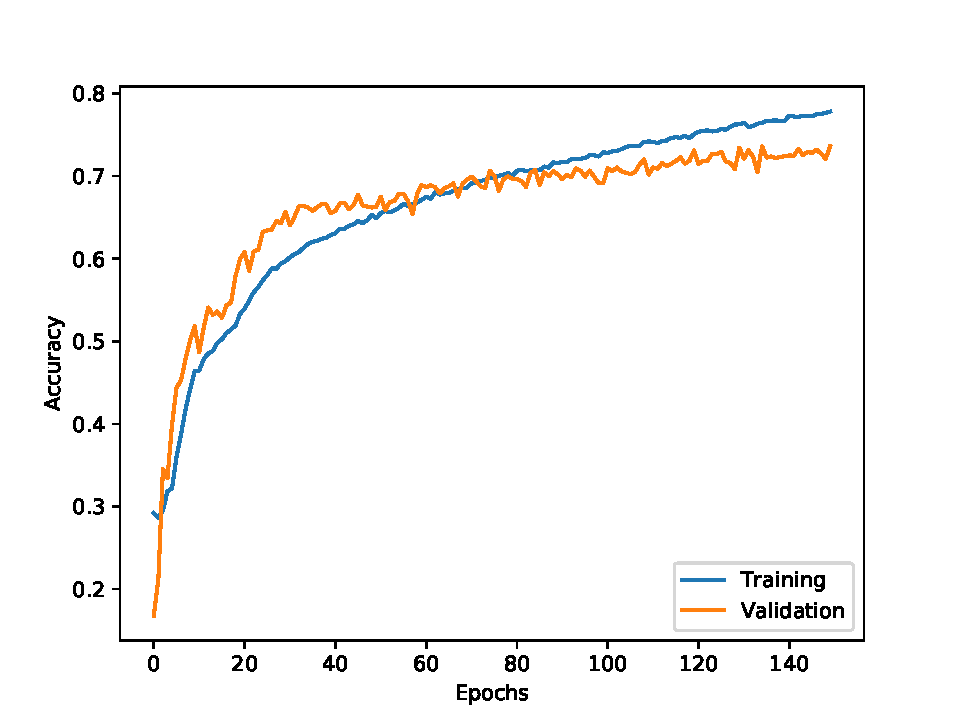
\includegraphics[width=5.5cm]{images/accuracy_history_scan_new.pdf}\hspace{0.5cm}
  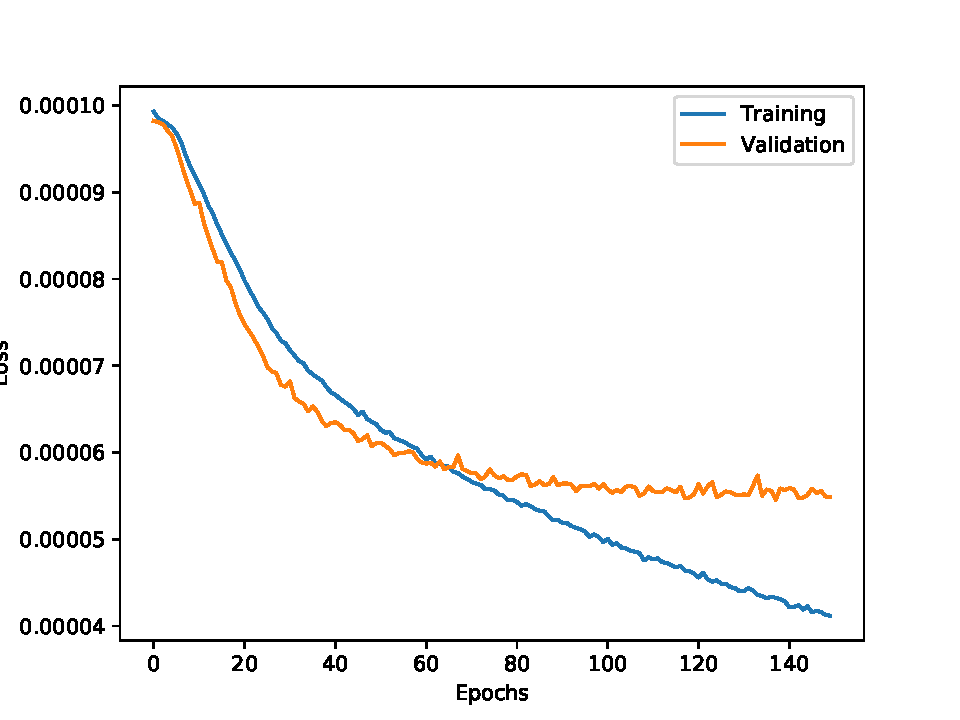
\includegraphics[width=5.5cm]{images/loss_history_scan_new.pdf} \\
 \end{figure}
\begin{itemize}
 \item[\textbullet] Sättigung ab ca. 80 Epochen auf dem Validierungsdatensatz
 \item[\textbullet] Erreicht ca. $71\,\%$ Genauigkeit beim Validierungsdatensatz
\end{itemize}


\end{frame}




\begin{frame}
 \frametitle{Performance des Referenznetzes}

 \begin{figure}
  \centering
  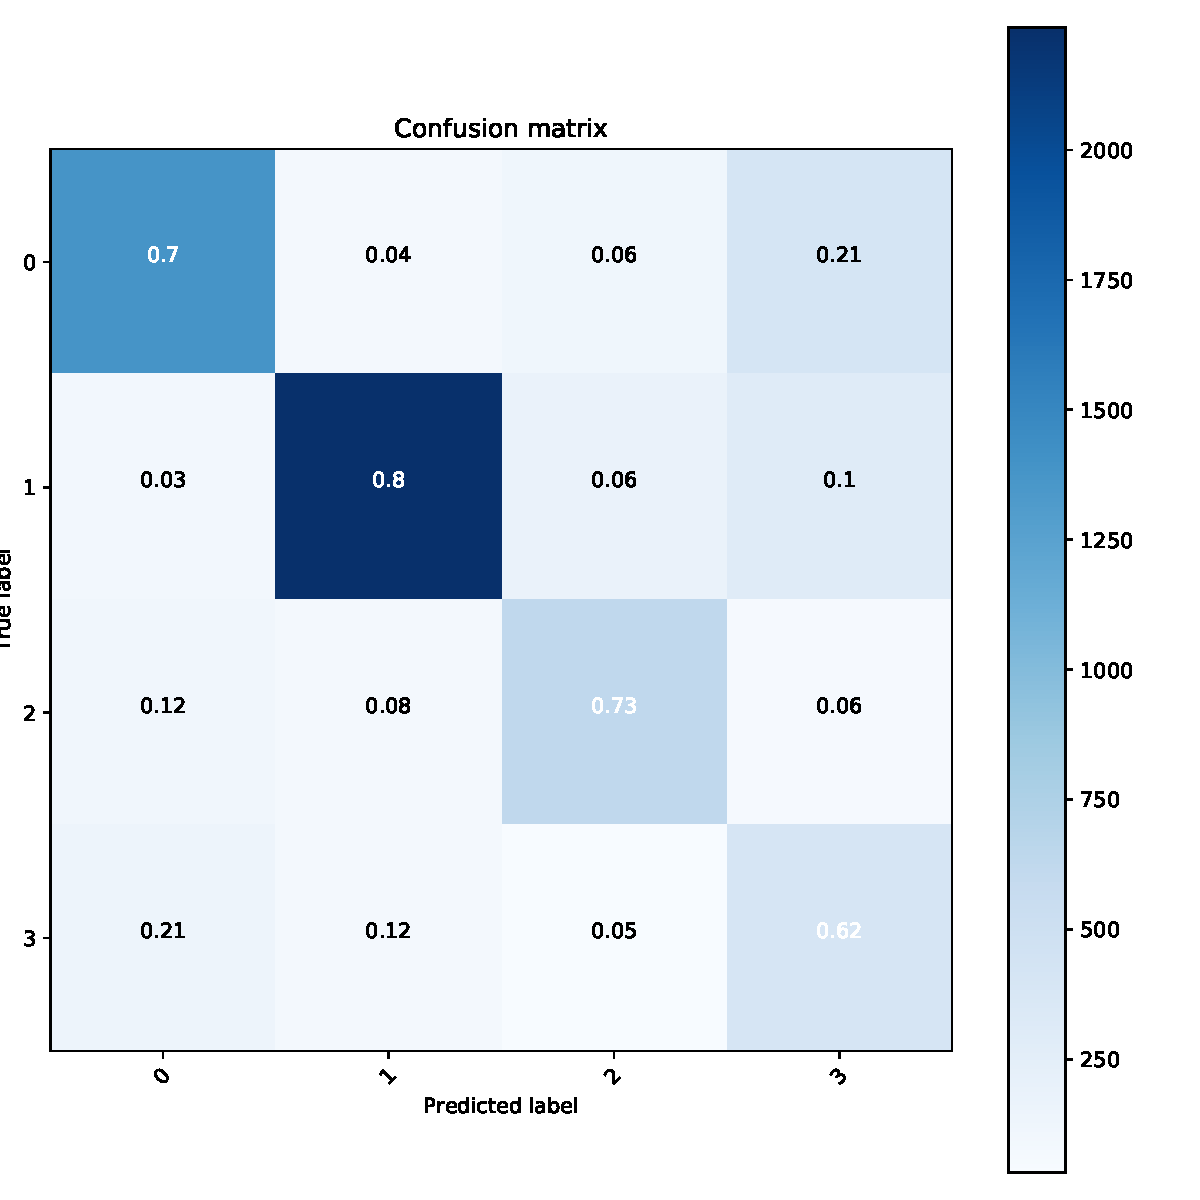
\includegraphics[width=5cm]{images/confusion_matrix_scan_new.pdf}\hspace{0.5cm}
  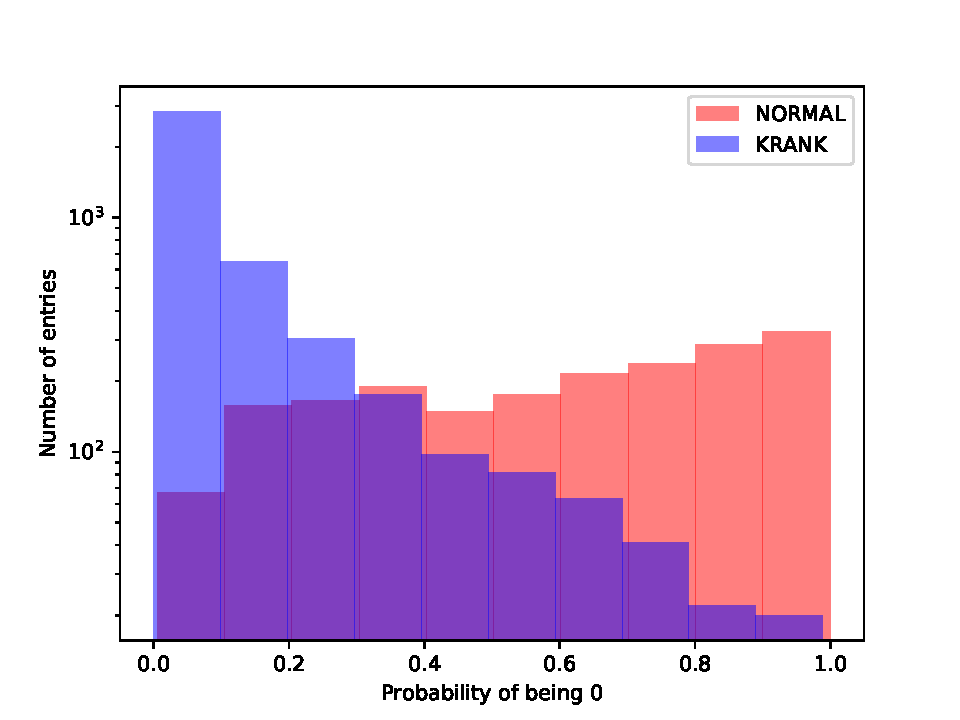
\includegraphics[width=5.5cm]{images/ill_or_not_scan_new.pdf}
 \end{figure}
\begin{itemize}
 \item[$\Rightarrow$] Gute Unterscheidung zwischen kranken und gesunden Augen möglich
 \item[$\Rightarrow$] Ähnliche Struktur der Verwirrungsmatrix wie bei nomineller Methode
\end{itemize}


\end{frame}


\begin{frame}
 \frametitle{Laufende Grid Search}
 \begin{itemize}
  \item[\textbullet] Optimierungsparameter:
  \begin{itemize}
   \item Batchgröße: 50, 64, 100, 128, 256, 512
   \item Aktivierungsfunktion: elu oder relu
   \item Outputaktivierungsfunktion: softmax oder sigmoid
   \item Layerstruktur (Dropout \& Dense)
  \end{itemize}
  \item[$\Rightarrow$] 120 verschiedene Netwerkkonfigurationen werden getestet
  \item[\textbullet] Modelle in .json und trainierte Gewichte in .hdf5 Files abgespeichert
  \vspace{0.5cm}
 \item[\textbullet] Erste Prognose: ca. $78\,\%$ ist drin
 \end{itemize}
\end{frame}

\end{document}
